
\chapter{Testes}
\label{cap:testes}

Testar é uma pratica intrínseca ao desenvolvimento e é antiga a necessidade de
criar programas para testar cenários específicos, de acordo com ~\citeonline{everett2007}.
%
Testes de software serão abordados neste capítulo, iniciando com uma visão geral de testes 
automatizados e conhecendo algumas práticas e padrões utilizados para desenvolver
os mesmos.

Para ~\citeonline{cotter1995} a automação de testes é uma prática ágil, eficaz e de baixo custo para melhorar
a qualidade dos sistemas de software. No entanto utilizar testes automatizados 
como uma premissa básica do desenvolvimento é um fenômeno relativamente recente, 
com início em meados  da década de 1990. Além do fato de ser uma técnica bastante utilizada pelas metodologias ágeis
de desenvolvimento.

%------------------------------------------------------------------------------%

\section{Testes Automatizados}

Teste automatizado é a prática de tornar os testes de software independentes da
intervenção humana, criando \textit{scripts} ou programas simples de computador que exercitam 
o sistema em teste, capturam os efeitos colaterais e fazem verificações, tudo 
automática e dinamicamente~\cite{meszaros2007}.
%
Os testes automatizados afetam diretamente a qualidade dos sistemas de software,
portanto, agregam valor  ao produto final, mesmo que os artefatos adicionais
produzidos não sejam visíveis para os usuários finais dos sistemas~\cite{bernardo2011}.

Será abordado neste trabalho o desenvolvimento de testes de aceitação para verificar sua relação com a usabilidade. 

\subsection{Testes de aceitação}

Os testes de aceitação, que possuem uma visão mais voltada para o usuário, fazem 
parte de uma fase do processo em que um teste de caixa-preta é realizado 
num sistema antes de sua disponibilização.
Para isso utilizamos o cucumber\footnote{\url{cukes.info}}, uma ferramenta que pode executar uma funcionalidades escrita em texto puro. Com base nas especificações da funcionalidade, o cucumber executa testes, proporcionando uma melhor comunicação entre equipe de desenvolvimento e cliente.
%
No cucumber, uma \textit{feature} é um requisito de alto nível 
expressado da perspectiva de uma pessoa e possui uma estrutura similar as histórias 
de usuário do XP~\cite{chelimsky2010}. 

Os testes de aceitação foram utilizados neste trabalho a fim de analisar possíveis influencias durante a inserção de práticas de usabilidade no desenvolvimento.


\subsection{Testes Funcionais e Unitários}
%
Os testes funcionais tem como objetivo no desenvolvimento na plataforma noosfero, verificar a integração da aplicação desenvolvida. Os testes unitários são executados em conjunto com os testes funcionais, porém  com o objetivo de verificar trechos menores de códigos. 

A descrição detalhada de testes de aceitação e de testes funcionais e unitários encontra-se no apêndice \ref{apendice2}.

\section{Técnicas de desenvolvimento de testes automatizados}

Automação de testes é uma técnica voltada principalmente para a melhoria de 
qualidade dos sistemas de software. 
%
No processo de desenvolvimento de software é fundamental controlar o custo do 
processo de testes, para isso baterias de testes automatizados devem ser bem 
definidas e implementadas. Assim, é importante conhecer boas práticas e técnicas 
de desenvolvimento de testes automatizados.    
%
Existem várias técnicas de desenvolvimento de software com testes que influenciam 
diretamente na qualidade do sistema. Essas técnicas geralmente possuem um processo 
de atividades pequeno e simples, como TDD e BDD.

\subsection{TDD - Test Driven Development}

Desenvolvimento dirigido por testes, TDD \textit{(Test-Driven Develepment)}, 
é uma técnica de desenvolvimento de software que se dá pela repetição disciplinada 
de um ciclo curto de passos de implementação de testes e do sistema~\cite{koskela2007}.
%
O ciclo de TDD é definido pelos seguintes passos:
%
\begin{enumerate}
\item Implementar um caso de teste;
\item Implementar um trecho do código suficiente para o novo caso de teste ter sucesso 
de tal modo que não quebre os testes previamente escritos;
\item Se necessário, refatorar o código produzido para que ele fique mais organizado;
\end{enumerate}

\begin{figure}[h]
    \centering
    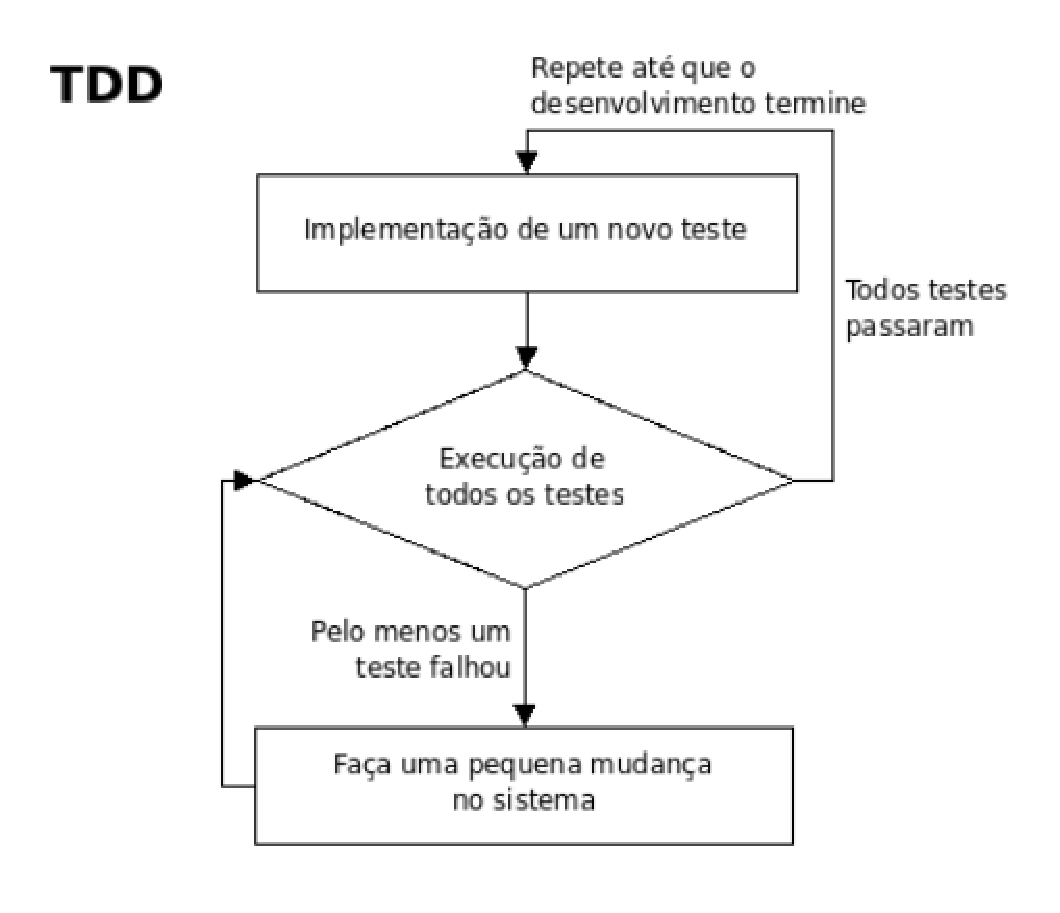
\includegraphics[keepaspectratio=true,scale=0.50]
      {figuras/tdd_ciclo.eps}
    \caption{Ciclo de atividades TDD~\cite{beck2002}}
    \label{tdd_ciclo}
\end{figure}

A técnica de desenvolvimento dirigido por testes foi definida por~\citeonline{beck2002}, como
representados na Figura~\ref{tdd_ciclo}.
%
Uma boa prática do TDD é a bateria de testes, que ajuda o desenvolvedor a evitar 
erros de regressão, quando o desenvolvimento de uma nova funcionalidade quebra uma 
já existente.
%
TDD também tende a contribuir com uma alta cobertura de código, uma 
fez que o desenvolvedor precisa escrever o testes antes da funcionalidade, 
possibilitando a criação de um código mais preciso, coeso e menos acoplado. 

Para ~\citeonline{massol2003}, o objetivo de TDD é código claro que 
funciona.
%
TDD propõe o desenvolvimento sempre em pequenos passo, deve-se escrever testes sempre 
para uma menor funcionalidade possível, escrever o código mais simples que faça o 
teste passar e fazer sempre apenas uma refatoração por vez~\cite{beck2002}. Assim o 
desenvolvedor se detém a criar soluções simples, sempre acompanhado de um constante 
\textit{feedback} dos testes.
%
O ciclo curto de passos definidos por TDD cria uma dependência forte entre codificação 
e testes, o que favorece e facilita a criação de sistemas com alta testabilidade~\cite{bernardo2011}. 
%
Índices altos de cobertura de código e testabilidade não garantem necessariamente 
qualidade do sistema, mas são métricas bem vistas para sistemas bem desenvolvidos.
%------------------------------------------------------------------------------%

\subsection{BDD - Behavior Driven Development}

Desenvolvimento dirigido por comportamento é uma prática que recomenda o mesmo ciclo de desenvolvimento de TDD, contudo, induzindo a utilização de uma linguagem ubíqua entre cliente e equipe de desenvolvimento, substituindo termos como assert, \textit{assert, test case, test suite} por termos mais comuns ao cliente, como \textit{should, context, specification}~\cite{bernardo2011}.

Embora seja principalmente uma ideia de como um processo de desenvolvimento de 
software deve ser gerenciado, a prática do BDD assume a utilização de ferramentas 
como suporte para o desenvolvimento de software~\cite{haring2011}. 
%
O BDD coloca em foco o comportamento em vez da estrutura de uma funcionalidade e faz isso em todos os níveis de desenvolvimento. Uma vez reconhecido isso, muda-se a forma de pensar sobre desenvolvimento para fora do código. Assim o foco parte para as interações, as pessoas e o sistema, sobre a 
estrutura do próprio sistema~\cite{chelimsky2010}.

Para que o comportamento seja analisado, é necessário entender o ponto de vista do 
cliente/usuário, entendendo o comportamento que o sistema deve ter a partir da
visão do cliente/usuário. 
%
De acordo com ~\citeonline{chelimsky2010}, estes são os três princípios do BDD:

\begin{enumerate}
\item \textbf{O suficiente é suficiente:} parte da ideia de gerenciar o esforço no 
planejamento inicial do sistema, para não fazer menos nem mais do que o necessário 
para começar, o que se aplica também ao processo de automação.

\item \textbf{Agregar valor às partes interessadas:} Se você está fazendo algo que 
não agrega valor ou que não aumenta a capacidade de agregar valor, pare e faça outra 
coisa em seu lugar.

\item \textbf{Tudo é comportamento:} Do código à aplicação, pode-se usar o mesmo 
pensamento e as mesmas construções linguísticas para descrever o comportamento, em 
qualquer nível de granularidade. 
\end{enumerate}

O comportamento do sistema é descrito em histórias de usuário, que são 
escritas com a participação tanto de clientes como desenvolvedores do sistema. 

Testes automatizados devem ser desenvolvidos com prioridade, buscando um rápido 
\textit{feedback}, contribuindo assim com a melhoria do sistema. Para isso é 
necessário que os cenários de testes estejam bem definidos junto à equipe.
%
 Considerando que o BDD se econtra bem adotado no ciclo de desenvolvimento deste estudo de caso, buscaremos nos próximos capítulos formas de abordar a usabilidade também no processo de desenvolvimento empírico, para na sequência mostrarmos o estudo de como relacionar as práticas de testes e as técnicas de usabilidade.

